% F1R3Beat — Game Design, version 2
% Build: xelatex f1r3beat-design.tex (twice). Brand fonts are read from ./fonts,
% logos from ./logos (both copied from github.com/F1R3FLY-io/f1r3fly-brand-portal).
\documentclass[11pt,a4paper]{article}

\usepackage[a4paper,top=30mm,bottom=26mm,left=22mm,right=22mm,headsep=10mm,footskip=12mm]{geometry}
\usepackage{fontspec}
\usepackage{xcolor}
\usepackage{graphicx}
\usepackage{tikz}
\usetikzlibrary{arrows.meta,positioning,calc,fit,backgrounds}
\usepackage{titlesec}
\usepackage{fancyhdr}
\usepackage{enumitem}
\usepackage{booktabs}
\usepackage{tabularx}
\usepackage{array}
\usepackage{listings}
\usepackage[most]{tcolorbox}
\usepackage{amsmath,amssymb}
\usepackage[hidelinks]{hyperref}
\usepackage{etoolbox}
\usepackage{microtype}

% ------------------------------------------------------------------ brand
% Colour system of 12 June 2026 (brand kit v1.2). White interior surface for a
% printable technical document: Yellow and Sky appear as rules and fills only,
% never as text, because both fail contrast as text on white.
\definecolor{brandyellow}{HTML}{F3D630}
\definecolor{brandsky}{HTML}{3FA9F5}
\definecolor{brandskydark}{HTML}{00528C}   % hue-locked Sky (205°), for links and outlines on white
\definecolor{brandblack}{HTML}{000000}
\definecolor{muted}{HTML}{3F3F3F}          % Neutral Gray, for secondary text on white
\definecolor{footgray}{HTML}{595959}
\definecolor{codebg}{HTML}{F2F2F2}
\definecolor{rulegray}{HTML}{C5C5C5}

\setmainfont{SourceSans3}[
  Path=./fonts/, Extension=.ttf,
  UprightFont=*-400, BoldFont=*-700, ItalicFont=*-400,
  ItalicFeatures={FakeSlant=0.18}, BoldItalicFont=*-700, BoldItalicFeatures={FakeSlant=0.18}]
\newfontfamily\spartanbold{LeagueSpartan-Bold}[Path=./fonts/, Extension=.ttf]
\newfontfamily\spartansemi{LeagueSpartan-SemiBold}[Path=./fonts/, Extension=.ttf]
\newfontfamily\spartanreg{LeagueSpartan-Regular}[Path=./fonts/, Extension=.ttf]
\newfontfamily\spartanlight{LeagueSpartan-Light}[Path=./fonts/, Extension=.ttf]
\newfontfamily\sourcelight{SourceSans3-300}[Path=./fonts/, Extension=.ttf]
\setmonofont{DejaVu Sans Mono}[Scale=0.84]
\renewcommand{\sffamily}{\spartanreg}

\newcommand{\caps}[1]{{\addfontfeatures{LetterSpace=12}\MakeUppercase{#1}}}
\newcommand{\gradrule}[1][\linewidth]{%
  \noindent\begin{tikzpicture}\shade[left color=brandyellow,right color=brandsky]
  (0,0) rectangle (#1,0.6pt);\end{tikzpicture}}

\hypersetup{colorlinks=true,linkcolor=brandskydark,urlcolor=brandskydark,citecolor=brandskydark,
  pdftitle={F1R3Beat: Game Design},pdfauthor={F1R3FLY.io}}

\titleformat{\section}{\spartanbold\fontsize{13}{16}\selectfont}
  {\caps{\thesection}\hspace{1em}}{0pt}{\caps}[\vspace{3pt}\gradrule]
\titleformat{\subsection}{\spartansemi\fontsize{10.5}{13}\selectfont}{\thesubsection\hspace{0.8em}}{0pt}{}
\titleformat{\subsubsection}[runin]{\bfseries}{}{0pt}{}[.]
\titlespacing*{\section}{0pt}{20pt}{12pt}
\titlespacing*{\subsection}{0pt}{14pt}{6pt}
\setcounter{secnumdepth}{2}
\setcounter{tocdepth}{1}

\setlength{\parindent}{0pt}
\setlength{\parskip}{6pt}
\linespread{1.08}
\emergencystretch=3em

\pagestyle{fancy}
\fancyhf{}
\renewcommand{\headrulewidth}{0pt}
\fancyhead[L]{\raisebox{-2pt}{\includegraphics[height=7.5mm]{logos/f1r3fly-io-horizontal-logo-white-background.pdf}}}
\fancyhead[R]{\spartanreg\fontsize{8}{10}\selectfont\color{footgray}\caps{F1R3Beat · Game design · v2}}
\fancyfoot[L]{\spartanbold\fontsize{7.5}{9}\selectfont\color{footgray}\thepage}
\fancyfoot[R]{\spartanbold\fontsize{7.5}{9}\selectfont\color{footgray}\textcopyright{} F1R3FLY INDUSTRIES, 2026. All Rights Reserved \textbar{} 6 October 2026}

\lstdefinelanguage{rholang}{
  morekeywords={new,in,for,contract,match,if,else,bundle,Nil,true,false,not,and,or},
  sensitive=true, morecomment=[l]{//}, morestring=[b]"}
\lstset{basicstyle=\ttfamily\small,backgroundcolor=\color{codebg},frame=leftline,
  rulecolor=\color{brandsky},framerule=1.2pt,framesep=6pt,xleftmargin=8pt,
  breaklines=true,columns=fullflexible,keepspaces=true,showstringspaces=false,
  keywordstyle=\bfseries,commentstyle=\color{muted},aboveskip=8pt,belowskip=8pt}

\newcommand{\code}[1]{\texttt{#1}}
\newcommand{\MUST}{\textsc{must}}
\newcommand{\MUSTNOT}{\textsc{must not}}
\newcommand{\SHOULD}{\textsc{should}}
\newcommand{\MAY}{\textsc{may}}

\newtcolorbox{decision}[2]{enhanced,breakable,colback=white,colframe=white,
  boxrule=0pt,left=10pt,right=4pt,top=4pt,bottom=4pt,
  borderline west={2.2pt}{0pt}{brandsky},
  fontupper=\small,
  title={\spartanbold\fontsize{8.5}{10}\selectfont\color{brandblack}\caps{Decision #1 · agreed}\quad
         \spartansemi\normalsize\fontsize{10.5}{12}\selectfont #2},
  coltitle=brandblack,colbacktitle=white,attach title to upper,after title={\par\smallskip}}

\newtcolorbox{finding}[2]{enhanced,breakable,colback=codebg,colframe=codebg,
  boxrule=0pt,left=8pt,right=6pt,top=5pt,bottom=5pt,arc=2pt,
  title={\spartanbold\fontsize{8.5}{10}\selectfont\caps{Finding #1}\quad\spartansemi\fontsize{10.5}{12}\selectfont #2},
  coltitle=brandblack,colbacktitle=codebg,attach title to upper,after title={\par\smallskip},fontupper=\small}

\newcounter{req}
\newcommand{\req}[1]{\refstepcounter{req}\label{#1}\textbf{R\thereq}}



\newtcolorbox{settled}[2]{enhanced,breakable,colback=white,colframe=white,
  boxrule=0pt,left=10pt,right=4pt,top=4pt,bottom=4pt,
  borderline west={2.2pt}{0pt}{brandyellow},
  fontupper=\small,
  title={\spartanbold\fontsize{8.5}{10}\selectfont\color{brandblack}\caps{Decision #1 · settled}\quad
         \spartansemi\normalsize\fontsize{10.5}{12}\selectfont #2},
  coltitle=brandblack,colbacktitle=white,attach title to upper,after title={\par\smallskip}}

\lstdefinelanguage{score}{
  morekeywords={score,import,pitches,durations,timbres,play,line,base,def,factor,pitchset,scale,gm,on,at,for,where},
  sensitive=true, morecomment=[l]{//}, morestring=[b]"}
% The body face has no small capitals, so RFC 2119 keywords are set in reduced capitals.
\renewcommand{\MUST}{{\fontsize{0.82em}{1em}\selectfont MUST}}
\renewcommand{\MUSTNOT}{{\fontsize{0.82em}{1em}\selectfont MUST NOT}}
\renewcommand{\SHOULD}{{\fontsize{0.82em}{1em}\selectfont SHOULD}}
\renewcommand{\MAY}{{\fontsize{0.82em}{1em}\selectfont MAY}}
\begin{document}

% ================================================================= cover
\begin{titlepage}
\newgeometry{margin=0pt}
\pagecolor{brandblack}\color{white}
\begin{tikzpicture}[remember picture,overlay]
  \node[anchor=north] at ($(current page.north)+(0,-38mm)$)
    {\includegraphics[width=70mm]{logos/f1r3fly-io-vertical-logo-color-on-dark.pdf}};
  \node[anchor=north west,text width=150mm,text=white] at ($(current page.north west)+(30mm,-150mm)$) {%
    {\spartanbold\fontsize{9}{11}\selectfont\color{brandyellow}\caps{F1R3Games · Game design}}\par\vspace{8mm}
    {\spartanlight\fontsize{40}{44}\selectfont F1R3Beat}\par\vspace{5mm}
    {\sourcelight\fontsize{15}{20}\selectfont Collective rhythmic intelligence on a F1R3FLY shard}\par\vspace{9mm}
    \begin{tikzpicture}\shade[left color=brandyellow,right color=brandsky] (0,0) rectangle (150mm,0.6pt);\end{tikzpicture}\par\vspace{7mm}
    {\fontsize{10.5}{15}\selectfont Version 2 \quad·\quad 6 October 2026\par
     Conforms to F1R3Node-Rust \code{master@95be0d4}, the F1R3Games Portal at \code{F1R3Games main@5937e4e},\par
     and the score calculus as implemented in \code{F1R3Score@76a355d}}};
  \node[anchor=south east] at ($(current page.south east)+(-22mm,14mm)$)
    {\spartanbold\fontsize{7.5}{9}\selectfont\color[HTML]{C5C5C5}\textcopyright{} F1R3FLY INDUSTRIES, 2026. All Rights Reserved \textbar{} 6 October 2026};
\end{tikzpicture}
\restoregeometry
\end{titlepage}
\nopagecolor\color{black}

% ================================================================= abstract
\begin{center}
\begin{minipage}{0.9\linewidth}
{\spartanbold\fontsize{8.5}{10}\selectfont\caps{Summary}}\par\smallskip
F1R3Beat is a multiplayer game in which a community makes a beat together. The board is a
grid: time runs left to right in columns, each a fixed subdivision of the beat, over a time
signature and a number of bars, all chosen when the game is set up, and each row is one instrument of a rock band. Each player
controls exactly one cell, and the only thing a player can do on the board is choose what that
cell plays: nothing, or one pitch from the row's palette. Players can also message one another
and send one another F1R3Cap. Any groove larger than one cell therefore has to be negotiated.

Patterns made in play are published to a gallery, and the ones people engage with most are
bred. A pattern is written as a score in the calculus of \emph{Scores as Processes}, as
implemented in F1R3Score: the beat is the parallel composition of its instruments' lines.
Reproduction is defined on those terms. A child takes one parent's rhythm and the other's
melody, row by row, or takes whole lines from each parent, so recombination happens exactly
where the score composes.

This document specifies the game against the stack as it stands on 6 October 2026. It
replaces the game installed with the Portal, an $8\times16$ sequencer in which any participant
could toggle any cell. It reuses the messaging and payments that the F1R3Pix design added to
the Portal. Version~2 records the review of 6 October 2026. All sixteen decisions in
Section~\ref{sec:decisions} are agreed. One changed in review: every note lasts one column,
and the column is chosen when the game is set up (D5).
\end{minipage}
\end{center}

\vspace{2mm}
\begingroup\small\setlength{\parskip}{0pt}\tableofcontents\endgroup
\newpage

% ================================================================= 1
\section{Purpose, sources and conformance}

\subsection{What the game is for}

F1R3Beat belongs to the F1R3Games suite of collective intelligence games, \emph{E Pluribus
Sapiens}. The suite's premise is that the actions of any one player are severely limited,
except for communication: anyone can talk to anyone, and everyone can see, or here hear, the
global result of the collective effort. Tokens generalise capital. They amplify or attenuate
what a player can achieve, and their first use is in negotiation.

F1R3Beat is cut from the same cloth as F1R3Pix. Where F1R3Pix makes coordination visible as
an image, F1R3Beat makes it audible as a groove. A kick on every beat, a backbeat on two and
four, or a bass figure that locks with the kick each needs several players to agree. The
original prototype already sketched the incentive: \emph{``I'll pay 100 F1R3Cap if we get
four-on-the-floor going.''}

F1R3Beat differs from F1R3Pix in one respect that shapes much of this document. Its plays
evolve. As with F1R3Skein's tunes, patterns that attract more engagement are selected more
often for reproduction, so the gallery is a population, and the community's taste acts on it
as selection pressure.

\subsection{Sources reviewed}

\begin{itemize}[leftmargin=1.2em,itemsep=2pt]
\item The original F1R3Beat design session (9 March 2026). It specified the rectangular grid,
  the time signature and bars, sixteenth-note steps, the rock-band timbres (bass, a standard
  drum set, guitar, keyboard, and a saxophone in place of vocals), one cell per player, and
  messaging and tokens as in F1R3Pix.
\item The music-snippet evolution session (3 March 2026) and \code{F1R3Skein/breeding}, which
  define F1R3Skein's breeding: engagement-weighted selection, the Mother/Father crossover of
  pitch and duration streams, padding by rests as mutation, and culling of the least engaged.
\item The design session of 6 October 2026, in which the author of the game settled the pitch
  palette, the single drum row, local tempo, and the use of F1R3Score's notation for
  reproduction (D4, D7 and D9 below), and the review of version~1 later that day, which agreed
  every decision, set note length by column (D5), and accepted the operators of D12 as
  workable for now.
\item The F1R3Games repository at \code{main@5937e4e}. It holds the March prototype
  (\code{F1R3Beat/UI}, \code{F1R3Beat/Shard}), the Portal (\code{Portal/f1r3games-portal}),
  and F1R3Pix as merged on 6 October: the client, the \code{seat}/\code{paint}/\code{say}
  environment, the Portal's \code{payments} domain, and host protocol 2.
\item The F1R3Pix design document, version 1 (5 October 2026), whose structure and many of
  whose decisions this document follows.
\item F1R3Score at \code{76a355d} (28 September 2026), the player for \emph{Scores as
  Processes}: its guide, \code{DESIGN.md}, \code{std.score} and examples. The player was built
  and run for this document. Every score in it was checked with \code{f1r3score check}, and
  the worked example was played with \code{f1r3score play}.
\item F1R3Node-Rust \code{master@95be0d4} and Embers \code{@28e50d4}, through the Portal and
  F1R3Pix designs.
\item The brand portal, \code{github.com/F1R3FLY-io/f1r3fly-brand-portal} at \code{283e00e}
  (brand kit v1.2), which governs this document's design.
\end{itemize}

\subsection{Order of authority}

Where sources disagree, this document follows the order the Portal design set: F1R3Node-Rust
\code{master}; then Embers; then F1R3Sky; then F1R3Gaze and ign1t10n; then the Portal and
F1R3Pix as merged on \code{main}. For the meaning of a score, F1R3Score is authoritative. The
March prototype and the earlier F1R3Games contracts are research. They are the record of what
the game is meant to be, and this document keeps their rules. It does not keep their storage,
signing or contract code.

\subsection{Conventions}

\MUST, \MUSTNOT, \SHOULD{} and \MAY{} are used as in RFC~2119. Requirements are numbered
R1, R2, \ldots{} and decisions D1, D2, \ldots. A \emph{participant} is an address in an
instance's \code{participants} map in the Portal environment. A \emph{seated} participant is
one who has been given a cell. A \emph{pattern} is the content of the board at one moment,
written as a score. A \emph{column} is the subdivision of the beat chosen when the game is set up, and a \emph{step} is one column. Durations are in whole notes, as in
F1R3Score.

% ================================================================= 2
\section{What the review found}\label{sec:findings}

\begin{finding}{1}{The installed game environment models a different game}
The Portal's \code{templates/games/f1r3beat.rho} defines \code{toggle(instance, voice, step,
on)} on a fixed pattern of 8 voices by 16 steps. Any participant may toggle any cell. That is a
shared drum machine. F1R3Beat has one cell per player, set only by its owner. The drift is the
same one F1R3Pix found: the \code{branding} branch rewrote the March prototype to a single
global grid, and the Portal followed that branch.
\end{finding}

\begin{finding}{2}{The pattern has no time signature or length}
The March design has the community pick a time signature and a number of bars, with each bar
measured in sixteenth notes. Every implementation since fixes the pattern at 16 steps.
\end{finding}

\begin{finding}{3}{Cells cannot carry a pitch, so the drum set took eight rows}
The prototype's cells are on or off. With no way to say which note a cell plays, the drum set
was spread over eight rows (kick, snare, hats, toms, clap, rim), and the bass, guitar, keyboard
and saxophone were never given rows at all. A pitched instrument cannot be played with a cell
that only says ``on''.
\end{finding}

\begin{finding}{4}{Tempo is a shared, global move}
The installed environment has \code{tempo(instance, bpm)}, which any participant can set for
everyone. The author of the game has settled that tempo is local to each listener (D7).
\end{finding}

\begin{finding}{5}{Messaging and payments now exist, and F1R3Beat can reuse them}
F1R3Pix, merged on 6 October, added sealed messages (\code{say}, \code{mail}, \code{outbox}),
the Portal environment's \code{payments.send} and \code{payments.list}, and host protocol 2
with \code{pay}, \code{open} and declared capabilities. None of these is specific to F1R3Pix.
F1R3Beat adopts them unchanged, with its own domain strings.
\end{finding}

\begin{finding}{6}{Breeding exists only in F1R3Skein's prototype}
\code{F1R3Skein/breeding/snippet-evolution.jsx} breeds snippets of two streams, pitches and
durations. Its children pair one parent's pitches with the other's durations, and two more
convert one parent's stream into the other kind by rewriting digits in base 5 or base 22. For
F1R3Beat, the Portal records only a \code{parents} field in the gallery header. No operator is
defined on a beat.
\end{finding}

\begin{finding}{7}{A shared keyboard does not keep a grid's time}
F1R3Score models a player at an instrument as a \emph{touch} (a message holding a duration)
sent to a \emph{key} (a receipt holding a pitch). That suggests one keyboard per row, with each
cell a touch entered at its step. Running that encoding showed why it fails. A key is one
receipt, so every touch waiting at it is in its contention set whatever its stamp, and the
contention set is resolved by weight, not by time. With touches at steps 0, 8 and 10 of one
kick, the player sounded the kick at steps 8, 10 and 11, not at step 0. A grid's cells
therefore become notes of a \emph{line}, one line per row, as \S\ref{sec:score} specifies. That
encoding plays every cell at its step.
\end{finding}

% ================================================================= 3
\section{The game}\label{sec:game}

\subsection{Rules}

\begin{enumerate}[leftmargin=1.4em,itemsep=3pt]
\item The arena is a grid with one row per instrument and one column per step of the
  subdivision. Its time signature, number of bars and column size are chosen when the instance
  is created and do not change.
\item Each participant may be \emph{seated} at exactly one cell, and each cell seats at most one
  participant. A cell with no one seated is \emph{void}. It is silent, unless the instance was
  seeded from a pattern (D16).
\item The only move on the board is \emph{set}: a seated participant chooses what their own
  cell plays: nothing, or one pitch from the row's palette. Every note lasts one column.
\item Off the board, any participant may send a message to any set of other participants, and
  may send F1R3Cap to any set of other participants.
\item Each player hears the pattern loop at a tempo of their own choosing. The tempo at which a
  player is listening is part of how other players see them.
\item Everything that happens on the board is recorded. The pattern at any moment can be
  published, and published patterns breed.
\end{enumerate}

There is no win condition inside a single game. Goals come from outside: from what the players
agree to make together, from the gallery's selection, or later from a tournament.

\subsection{The grid}

The rows are fixed in this version, in this order from top to bottom:

\begin{center}\small
\begin{tabularx}{\linewidth}{@{}l l l l X@{}}
\toprule
row & index & timbre & F1R3Score declaration & range\\
\midrule
\code{drums}  & 0 & General MIDI percussion       & \code{drums = gm(0) on 10}  & the 12 pieces of the kit (Table~\ref{tab:kit})\\
\code{bass}   & 1 & Electric bass (finger)        & \code{bass = gm(33) on 2}   & E1--G3 (MIDI 28--55)\\
\code{guitar} & 2 & Overdriven guitar             & \code{guitar = gm(29) on 3} & E2--E5 (40--76)\\
\code{keys}   & 3 & Acoustic grand piano          & \code{keys = gm(0) on 4}    & C2--C6 (36--84)\\
\code{sax}    & 4 & Tenor saxophone               & \code{sax = gm(66) on 5}    & G\#2--D\#5 (44--75)\\
\bottomrule
\end{tabularx}
\end{center}

A column has length $u$ whole notes, chosen from $1/4$, $1/8$, $1/16$ and $1/32$ and the triplet
subdivisions $1/6$, $1/12$ and $1/24$. A time signature $n/d$ with column $u$ gives $n/(du)$
steps per bar, which must be a whole number. With $b$ bars the pattern has $S=nb/(du)$ steps and
$5S$ cells. A cell is addressed by its step $t$ and row
$\rho$, and its index is $c=5t+\rho$, so cells are numbered in time order and simultaneous cells
are adjacent. That order is the one encodings use, and the one keyboard navigation follows.

\begin{center}\small
\begin{tabular}{@{}lccccccc@{}}
\toprule
time signature & 4/4 & 3/4 & 6/8 & 7/8 & 5/4 & 12/8 & 2/4\\
steps per bar, $u=1/8$   & 8 & 6 & 6 & 7 & 10 & 12 & 4\\
steps per bar, $u=1/16$  & 16 & 12 & 12 & 14 & 20 & 24 & 8\\
cells, $u=1/16$, 2 bars  & 160 & 120 & 120 & 140 & 200 & 240 & 80\\
cells, $u=1/16$, 4 bars  & 320 & 240 & 240 & 280 & --- & --- & 160\\
\bottomrule
\end{tabular}
\end{center}

\begin{decision}{D1}{How large is the grid, and what are empty cells?}
\textbf{Options.} (a) The host fixes the shape and a capacity $N\le 5S$ at creation, and
unseated cells are void. (b) The grid grows by a bar when it fills. (c) The grid has exactly as
many cells as there are players.

\textbf{Agreed: (a).} A groove is planned against a fixed loop, and (b) and (c) would
change its length during play. Void cells are silence, and silence is most of any good beat:
a full grid is a wall of sound. The default is 4/4 in sixteenth-note columns, 2 bars, and a capacity of 32, so one cell in
five can sound. The bound is $S\le 64$ steps (320 cells) in this version, so that a whole-grid
read stays one explore deploy of modest cost. Phase~4 of the plan measures it.
\end{decision}

\subsection{Seating}

\begin{decision}{D2}{Who chooses where a player sits?}
\textbf{Options.} (a) Random: the environment assigns a cell. (b) Claim: the player chooses a
free cell. (c) Row: the player chooses an instrument, and the environment assigns a free step in
that row at random.

\textbf{Agreed: (a) by default, with (b) and (c) as host options.} Random seating
keeps where a player sits out of their hands, as in F1R3Pix, so neighbours who have never met
must still negotiate. Row seating is new and suits music: a bassist can choose to play bass
without choosing their moment. Claim seating suits games among friends and tournaments with set
formations.

\textbf{Random seating, precisely.} As in F1R3Pix, with cell indices in place of spiral indices.
Let $h=\mathrm{blake2b256}(\mathit{instance}\,\|\,\mathit{address})$, read as an unsigned
integer. Starting at index $h\bmod 5S$, the environment takes the first free cell in
increasing index order, wrapping at the end. Row seating does the same within the row's cells
$\{5t+\rho\}$, starting at step $h\bmod S$. Either result can be checked by anyone.
\end{decision}

\begin{decision}{D3}{What happens to a cell when its player leaves?}
\textbf{Agreed: as F1R3Pix D3.} The cell stays owned and keeps playing its last note.
The client draws it dimmed, and rejoining restores control.
\end{decision}

\subsection{Pitch}

\begin{settled}{D4}{A cell plays one pitch from its row's palette}
Settled on 6 October 2026: as in F1R3Pix, where a cell takes a colour, a cell in F1R3Beat takes
a pitch from a palette. The drum set is therefore a single row, whose palette is the pieces of
the kit. That also reduces the grid's height from the prototype's eight drum rows plus four
instruments to five rows.

\textbf{What follows from it.} A pitched row's palette is every pitch in its range. The host may restrict the pitched rows to a scale, written as F1R3Score writes
one: a kind (\code{major}, \code{minor}, \code{dorian}, \code{pentatonic},
\code{minor-pentatonic}, \code{blues} or \code{chromatic}) and a tonic. A row's palette is then
the scale's pitches within the row's range. The drum row is unaffected by the scale. Pitches
are written in scientific notation with sharps (\code{C\#3}), as F1R3Score names MIDI numbers.
Kit pieces are written by name. One cell plays one note, so each row is monophonic, and harmony
comes from the rows sounding together.
\end{settled}

\begin{table}[h]
\centering\small
\begin{tabular}{@{}llr@{\qquad}llr@{\qquad}llr@{}}
\toprule
name & piece & MIDI & name & piece & MIDI & name & piece & MIDI\\
\midrule
\code{kick}  & bass drum   & 36 & \code{chh}  & closed hi-hat & 42 & \code{ltom}  & low tom      & 45\\
\code{rim}   & side stick  & 37 & \code{phh}  & pedal hi-hat  & 44 & \code{mtom}  & low-mid tom  & 47\\
\code{snare} & snare       & 38 & \code{ohh}  & open hi-hat   & 46 & \code{htom}  & high tom     & 50\\
\code{clap}  & hand clap   & 39 & \code{crash}& crash cymbal  & 49 & \code{ride}  & ride cymbal  & 51\\
\bottomrule
\end{tabular}
\caption{The kit. Names are F1R3Score pitch identifiers with explicit MIDI numbers on the
General MIDI percussion channel.}
\label{tab:kit}
\end{table}

\subsection{How long a note lasts}

\begin{settled}{D5}{A note lasts one column, and the column is set when the game begins}
Settled in review on 6 October 2026: note length is decided by column size. A column
determines the subdivision of the beat, and it is chosen when the game is set up, together with
the time signature and the number of bars. Every note lasts exactly one column.

\textbf{What follows from it.} No row holds its notes, and no palette contains a rest: a cell
plays one pitch or nothing. A longer sound is a choice of subdivision, not a property of a
row, so a host who wants longer notes chooses a coarser column. The map from a grid to its
score is injective (R\ref{r:canon}). The column is part of a pattern's shape, so it joins the
meter in deciding which patterns can breed (D13), and a seed must match it (D16). Notes longer
than one column, written as ties across cells, are left for a later version.
\end{settled}

\subsection{Phases}

\begin{decision}{D6}{What may players do in each phase?}
\textbf{Agreed: as F1R3Pix D5, with \code{listen} beside \code{seat}.}

\begin{tabular}{@{}lcccccc@{}}
\toprule
 & seat & set & listen & message & pay & read \\
\midrule
\code{lobby}  & yes & no  & yes & yes & yes & yes\\
\code{active} & yes & yes & yes & yes & yes & yes\\
\code{closed} & no  & no  & no  & no  & no  & yes\\
\bottomrule
\end{tabular}
\end{decision}

\subsection{Tempo}

\begin{settled}{D7}{Tempo is local to each listener}
Settled on 6 October 2026: an instance has a default tempo, but changing the tempo is a local
move. Player A can listen at a different tempo from player B. The tempo a player is listening
at is a description of the player: \emph{listening at 92~bpm}.

\textbf{What follows from it.} Tempo is not part of the pattern. It is not in the grid or in
the score, and two patterns that differ only in the tempo they were heard at are the same
pattern. This matches F1R3Score, in which a score is written in whole notes and \code{--bpm} is
a rendering parameter only. The host sets the default (100~bpm unless changed, within
40--240). Each player's listening tempo is published on the chain, so that it can be seen, by
the \code{listen} move (\S\ref{sec:env}). A published pattern carries its publisher's listening
tempo as a suggestion, and every listener can override it. The installed \code{tempo} move is
retired.
\end{settled}
% ================================================================= 4
\section{Architecture}\label{sec:arch}

F1R3Beat adds one new kind of component to what F1R3Pix uses: a \emph{breeder}, which runs the
gallery's evolution. Everything else is one game environment on the shard, one game client
framed by the Portal shell, and the Portal's existing \code{payments} domain and host protocol
2. The score bridge, the code that turns a grid into a score, is a library shared by the client,
the breeder and anyone who audits them.

\begin{figure}[ht]
\centering
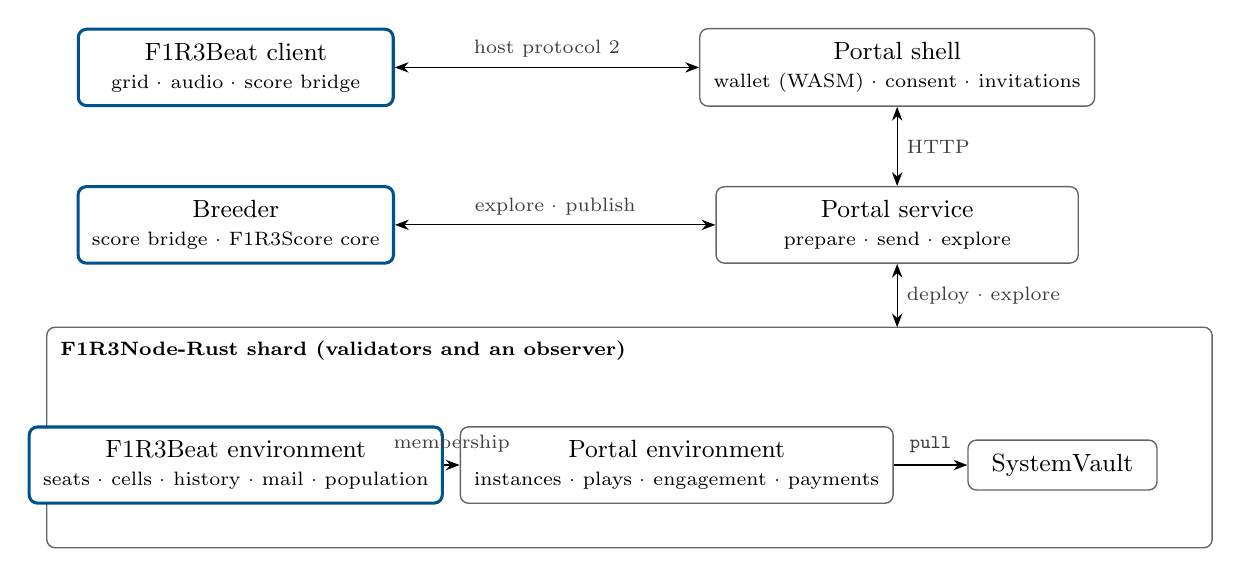
\begin{tikzpicture}[font=\small,
  box/.style={draw=black!60,line width=0.5pt,rounded corners=3pt,align=center,inner sep=5pt,fill=white},
  new/.style={box,draw=brandskydark,line width=1.1pt},
  lab/.style={font=\scriptsize,text=muted,align=center},
  >={Stealth[length=5pt]}]
  \node[new,minimum width=40mm] (game) at (0,0) {F1R3Beat client\\[-1pt]{\scriptsize grid · audio · score bridge}};
  \node[box,minimum width=46mm] (shell) at (8.4,0) {Portal shell\\[-1pt]{\scriptsize wallet (WASM) · consent · invitations}};
  \node[box,minimum width=46mm] (svc) at (8.4,-2.0) {Portal service\\[-1pt]{\scriptsize prepare · send · explore}};
  \node[new,minimum width=40mm] (breed) at (0,-2.0) {Breeder\\[-1pt]{\scriptsize score bridge · F1R3Score core}};
  \draw[black!60,rounded corners=3pt,line width=0.5pt] (-2.4,-3.3) rectangle (12.4,-6.1);
  \node[anchor=north west,font=\scriptsize\bfseries] at (-2.35,-3.35) {F1R3Node-Rust shard (validators and an observer)};
  \node[new,minimum width=36mm] (benv) at (0,-5.05) {F1R3Beat environment\\[-1pt]{\scriptsize seats · cells · history · mail · population}};
  \node[box,minimum width=40mm] (penv) at (5.6,-5.05) {Portal environment\\[-1pt]{\scriptsize instances · plays · engagement · payments}};
  \node[box,minimum width=24mm] (vault) at (10.5,-5.05) {SystemVault};
  \draw[<->] (game) -- node[above,lab]{host protocol 2} (shell);
  \draw[<->] (shell) -- node[right,lab]{HTTP} (svc);
  \draw[<->] (svc) -- node[right,lab]{deploy · explore} (8.4,-3.3);
  \draw[<->] (breed) -- node[above,lab]{explore · publish} (svc);
  \draw[->] (benv) -- node[above,lab,yshift=1pt]{membership} (penv);
  \draw[->] (penv) -- node[above,lab,yshift=1pt]{\code{pull}} (vault);
\end{tikzpicture}
\caption{Components. Outlined in dark sky: what this design adds or replaces.}
\label{fig:arch}
\end{figure}

\subsection{Authority}

The design keeps the Portal's separation of authority, as F1R3Pix does.

\begin{itemize}[leftmargin=1.2em,itemsep=2pt]
\item The game client never sees a key. It reaches identity, the shard and payment only
  through the host protocol.
\item The F1R3Beat environment reads two things and nothing else: the caller's address,
  which it obtains from \code{rho:deploy:data} through \code{rho:vault:address}, and the block
  height, from \code{rho:block:data}. It never touches a vault.
\item Funds move only through the Portal environment's \code{payments.send}, signed only from
  the Portal shell after a prompt.
\item The breeder holds one key, the \emph{breeder key}, registered in the F1R3Beat environment
  by the F1R3FLY.io Cooperative. That key can admit patterns to the population and remove them,
  and nothing else. Everything it does is recomputable from public data (\S\ref{sec:evolution}).
\end{itemize}

% ================================================================= 5
\section{The F1R3Beat environment}\label{sec:env}

The environment replaces the installed \code{f1r3beat.rho} body inside the shared game
\code{prelude.rho}, keeping the prelude's machinery (installation under the game's registry
key, version-checked upgrade, \code{who}, \code{member}, \code{instanceOf}, \code{TreeHashMap}).
Its moves follow F1R3Pix's moves one for one. \code{set} plays the part of \code{paint}, and
\code{listen} is new. Installing it raises the environment version. The URI is unchanged and
every call template's hash changes, so the manifest is re-registered (\S\ref{sec:manifest}).

\subsection{Configuration}

The configuration is the \code{config} map the host passes to the Portal's
\code{instances.create}. The environment reads it from the Portal's instance record.

\begin{lstlisting}[language=rholang]
{ "meter":   [4, 4],         // n/d, with n/(d*column) a whole number
  "bars":    2,              // S = n*bars/(d*column) steps, 1 <= S <= 64
  "capacity": 32,            // 1 ..= 5*S                                      (D1)
  "seating": "random",       // "random" | "claim" | "row"                     (D2)
  "scale":   Nil,            // Nil, or ["minor-pentatonic", "E"]              (D4)
  "column":  [1, 16],         // 1/4, 1/8, 1/16, 1/32, 1/6, 1/12, 1/24          (D5)
  "tempo":   100,            // default listening tempo, 40 ..= 240            (D7)
  "seed":    Nil,            // Nil, or a seeding pattern                       (D16)
  "messageLimit": 2048 }     // bytes of sealed envelope per message
\end{lstlisting}

\req{r:config}~The environment \MUST{} refuse every move on an instance whose configuration is
missing or out of range, answering \code{(false, "bad config")}. It \MUSTNOT{} substitute
defaults. Defaults are applied by the client that creates the instance, where the host can see
them.

\subsection{State}

\begin{center}\small
\begin{tabularx}{\linewidth}{@{}>{\ttfamily}p{27mm} X >{\raggedright\arraybackslash}p{24mm}@{}}
\toprule
\normalfont key & value & written by\\
\midrule
("seat", i, a)  & \code{\{"cell": c, "pk", "listen": bpm, "at", "h"\}} & \code{seat}, \code{listen}, by $a$\\
("cell", i, c)  & \code{\{"owner": a | Nil, "note": v, "at", "h", "n"\}} & \code{seat}, \code{set}\\
("hist", i, c)  & list of \code{[h, ts, v]}, oldest first & \code{set}\\
("out", i, a)   & sealed envelopes, as F1R3Pix & \code{say}, by $a$\\
("pop", p)      & \code{\{"meter", "steps", "born", "origin"\}} & breeder key\\
\bottomrule
\end{tabularx}
\end{center}

A cell's note $v$ is \code{Nil} (plays nothing) or a pitch name from the row's palette. Seeded cells that no one occupies have
owner \code{Nil} and keep their seeded note (D16).

\req{r:single-writer}~After seating, every key \code{("cell", i, c)}, \code{("hist", i, c)},
\code{("seat", i, a)} and \code{("out", i, a)} has exactly one writer. Players setting notes,
changing tempo or messaging never contend for a key. There is deliberately no instance-wide
counter or log.

\subsection{Moves}

Moves are play templates, signed within the allowance granted at launch. Each answers
\code{(true, value)} or \code{(false, reason)}.

\textbf{\code{seat(instance, pk, want)}.} As F1R3Pix's \code{seat}. \code{want} is \code{Nil}
under random seating, a cell index under claim seating, or a row index under row seating. The
key \code{pk} is checked against the caller's address with \code{rho:vault:address}'s
\code{"fromPublicKey"}. A new seat's \code{listen} is the instance's default tempo. Seating on a
seeded cell takes ownership of it without changing its note. Answers the cell index.

\textbf{\code{set(instance, note)}.} Sets what the caller's own cell plays. Like
\code{paint}, the move names no cell.
\begin{itemize}[leftmargin=1.2em,itemsep=1pt]
\item Refuses unless the caller is a participant, the status is \code{active}, and the caller
  is seated.
\item Refuses unless \code{note} is \code{Nil} or a member of the palette of the caller's row
  (D4).
\item Writes the cell with \code{n} incremented, appends \code{[h, ts, note]} to its history,
  and answers \code{\{"cell": c, "note": note, "h": h\}}.
\end{itemize}

\textbf{\code{listen(instance, bpm)}.} Records the tempo the caller is listening at. It refuses
unless the caller is seated, the status is not \code{closed}, and $40\le\mathit{bpm}\le 240$ is
an integer. It changes nothing anyone hears but the caller. The client debounces it, so it
publishes a tempo only once the slider has rested for two seconds.

\textbf{\code{say(instance, to, envelope)}.} As F1R3Pix's \code{say}.

The breeder key has two further moves, described in \S\ref{sec:evolution}: \code{admit} and
\code{cull}.

\subsection{Reads}

\begin{center}\small
\begin{tabularx}{\linewidth}{@{}>{\ttfamily}l X@{}}
\toprule
\normalfont template & answers\\
\midrule
f1r3beat.grid(instance)     & the configuration, the status, and every non-void cell with owner, note, \code{at}, \code{h} and \code{n}\\
f1r3beat.seats(instance)    & map from address to \code{\{"cell", "pk", "listen"\}}\\
f1r3beat.log(instance, from, to) & every \code{set} with $\mathit{from}\le h<\mathit{to}$, as \code{[h, ts, owner, c, v]}, in history order\\
f1r3beat.mail(instance, address, cursor) & as F1R3Pix\\
f1r3beat.outbox(instance, address, from) & as F1R3Pix\\
f1r3beat.population(cursor) & population members after \code{cursor}, with their records\\
\bottomrule
\end{tabularx}
\end{center}

Every read result carries the block hash it reflects. History is ordered by height, then
timestamp, then owner address, then the order of sets within a cell, as in F1R3Pix.

\subsection{A sketch of \code{set}}

\begin{lstlisting}[language=rholang]
contract env(@"set", @instance, @note, ret) = {
  new whoCh, rCh, sCh, hCh, okCh, ack1, ack2 in {
    who!(*whoCh) |
    for (@by, @ts <- whoCh) {
      ready!(instance, by, "active", *rCh) |      // participant, status, config
      for (@ok, @why <- rCh) {
        if (not ok) { ret!((false, why)) } else {
          TreeHashMap!("get", state, ("seat", instance, by), *sCh) |
          for (@seat <- sCh) {
            match seat {
              Nil => { ret!((false, "take a seat first")) }
              _ => { match seat.get("cell") { c => {
                allowed!(instance, c, note, *okCh) |   // palette of row c % 5
                for (@fits <- okCh) {
                  if (not fits) { ret!((false, "not in this row's palette")) } else {
                    height!(*hCh) |
                    for (@h <- hCh) {
                      update!(("cell", instance, c), note, ts, h, *ack1) |
                      append!(("hist", instance, c), [h, ts, note], *ack2) |
                      for (_ <- ack1 & _ <- ack2) {
                        ret!((true, {"cell": c, "note": note, "h": h}))
                      }
                    }
                  }
                }
              } } }
            }
          }
        }
      }
    }
  }
}
\end{lstlisting}

\code{allowed} computes a row's palette from the configuration once per instance and keeps it
under \code{("palette", i, row)}, written at the instance's first seat. The palette of a pitched
row is at most 49 pitches, so the check is a set lookup.

% ================================================================= 6
\section{Messages and payments}\label{sec:mail}

\begin{decision}{D8}{How do players talk and pay?}
\textbf{Agreed: exactly as F1R3Pix (its D6, D7 and D10).} Messages are on the chain and
sealed to their recipients and the sender, with the domain strings \code{"f1r3beat/msg/v1"} in
place of F1R3Pix's. Payments go through the Portal environment's \code{payments.send}, signed
only from the shell after a prompt, with \emph{each} as the default and \emph{split} on
request. The manifest declares \code{"capabilities": ["pay", "open"]}. Nothing in either
mechanism is specific to F1R3Pix, and reusing it means the second game to use it proves that.
\end{decision}

The same requirements apply: the host binds the game id and instance into \code{open}
(F1R3Pix R4), refuses a \code{pay} naming a non-participant before prompting (F1R3Pix R7), and
never signs \code{payments.send} within an allowance (F1R3Pix R6).

% ================================================================= 7
\section{From grid to score}\label{sec:score}

\begin{settled}{D9}{Patterns are written, and reproduce, in F1R3Score's notation}
Settled on 6 October 2026: the recombination operator for F1R3Beat uses the notation system of
F1R3Score. This section gives the encoding. \S\ref{sec:evolution} defines reproduction on it.
\end{settled}

\subsection{The shape of the score}

A pattern is the parallel composition of five lines, one per row. Each line is the sequence of
the notes and rests that its row plays, in F1R3Score's \code{line} form: a right-nested chain of
written notes, each a key on a pitch channel and a touch on a duration co-channel that meet and
play. The components in composition are therefore the instruments, and the composition is the
beat. Each line's durations add up to the length of the pattern, so the five lines start
together and end together, and the pattern loops.

\begin{figure}[h]
\centering
\begin{tikzpicture}\input{fig/mother.tex}\end{tikzpicture}
\caption{A pattern in 4/4, one bar, in sixteenth-note columns. Each sounding cell is a note one
column long. The keys row plays nothing.}
\label{fig:mother}
\end{figure}

\begin{lstlisting}[language=score,basicstyle=\ttfamily\scriptsize]
// F1R3Beat pattern, canonical form v2 · meter 4/4 · bars 1 · column 1/16 · columns 16
score F1R3Beat
import std
pitches   { r, kick = 36, snare = 38, chh = 42, ohh = 46, E2, G2, A2, D3, E3, D4, E4 }
durations { c1 = 1/16, c2 = 1/8, c3 = 3/16, c4 = 1/4, c7 = 7/16, c16 = 1 }
timbres   { drums = gm(0) on 10, bass = gm(33) on 2, guitar = gm(29) on 3,
            keys = gm(0) on 4, sax = gm(66) on 5 }
play line(base "drums", drums)       [ kick c1, r c1, chh c1, r c1, snare c1, r c1, chh c1, r c1,
                                     kick c1, r c1, kick c1, r c1, snare c1, r c1, ohh c1, r c1 ]
   | line(base "bass", bass)         [ E2 c1, r c2, E2 c1, r c2, G2 c1, r c1, A2 c1, r c2,
                                     A2 c1, r c4 ]
   | line(base "guitar", guitar)     [ r c4, E3 c1, r c7, D3 c1, r c3 ]
   | line(base "keys", keys)         [ r c16 ]
   | line(base "sax", sax)           [ r c4, D4 c1, r c3, E4 c1, r c7 ]
\end{lstlisting}

This is the pattern of Figure~\ref{fig:mother}. \code{f1r3score check} accepts it (digest
\code{1fc69fbb\ldots}), and \code{f1r3score play} plays every note at its column: kick and bass
at 0, the closed hat at $1/8$, the second bass note at $3/16$, snare, guitar and saxophone at
$1/4$, and so on.

\subsection{Canonical form}\label{sec:canonical}

Breeding, deduplication and verification all compare patterns, so the score of a grid must be
unique. F1R3Score's structural digest depends on the declarations as well as on the play term,
including the order of the alphabets. The \emph{canonical form} fixes every choice.

\begin{enumerate}[leftmargin=1.4em,itemsep=2pt]
\item \textbf{Lines.} For each row, in the order drums, bass, guitar, keys, sax, read the cells
  $v_0,\dots,v_{S-1}$. Each pitch $v_t$ is the note $(v_t,u)$. Each maximal run of silent cells
  is one rest \code{r}, as long as the run. A row with no notes is the single rest
  \code{[ r c$S$ ]}.
\item \textbf{Durations.} A length of $k$ columns is named \code{c$k$} $=ku$, written in
  lowest terms. Exactly the lengths used are declared, in increasing order.
\item \textbf{Pitches.} \code{r} first; then the kit pieces used, in increasing MIDI
  order (Table~\ref{tab:kit}); then the pitched notes used, in increasing MIDI order, in scientific
  notation with sharps.
\item \textbf{Timbres.} All five declarations, always, as in the table of \S\ref{sec:game}.
\item \textbf{Text.} The score is named \code{F1R3Beat} and imports \code{std}. The first line
  is the comment shown above. Layout is the one shown: two spaces of indentation, \code{|} at
  the start of each line after the first, and a single space after each comma.
\end{enumerate}

\req{r:canon}~The score bridge \MUST{} produce the canonical form, and a pattern's identity is
the F1R3Score digest of its canonical score. Because every note is one column long, two grids of
one shape have the same digest exactly when they play the same notes.

\subsection{What the score is used for}

\begin{itemize}[leftmargin=1.2em,itemsep=2pt]
\item \textbf{The gallery.} A pattern play's body is its canonical score (\S\ref{sec:gallery}),
  so a published pattern can be played by \code{f1r3score} with no F1R3Beat code at all, and
  rendered to MIDI with \code{f1r3score play --midi}.
\item \textbf{Identity.} The digest names the pattern. It deduplicates the population and
  links a child to its parents.
\item \textbf{The genome.} Reproduction is defined on lines and on the composition of lines
  (\S\ref{sec:evolution}).
\item \textbf{Playback.} The client plays the notes the score denotes. Conformance tests check
  that the client's note list is the one \code{f1r3score play --format json} reports, rests
  excluded (\S\ref{sec:manifest}).
\end{itemize}

\subsection{Why lines and not keyboards}

F1R3Score's instruments separate the player from the instrument: a key, holding a pitch,
belongs to the instrument, and a touch, holding a duration, belongs to the player. That reading
fits a game of players at instruments, and it was the first encoding tried. As Finding~7
records, it does not keep a grid's time, because touches waiting at one key contend whatever
their stamps. A line is sequential composition. Each note's continuation is stamped at the end
of the note before it, so time is exact.

What the line form loses is a record, inside the score, of which player played which note. The
gallery keeps that separately, as the play's credits (\S\ref{sec:gallery}). When F1R3Score
gains a timed touch, the keyboard form can be revisited (\S\ref{sec:future}).
% ================================================================= 8
\section{The client}\label{sec:client}

The client follows F1R3Pix's: a web page from the game's own origin, framed by the Portal, with
a framework-free core holding every operation and a React layer that only renders. The core
adds two modules to F1R3Pix's: the TypeScript score bridge (grid to canonical score, and score
to notes), and the audio engine.

\subsection{Layout}

\begin{figure}[h]
\centering
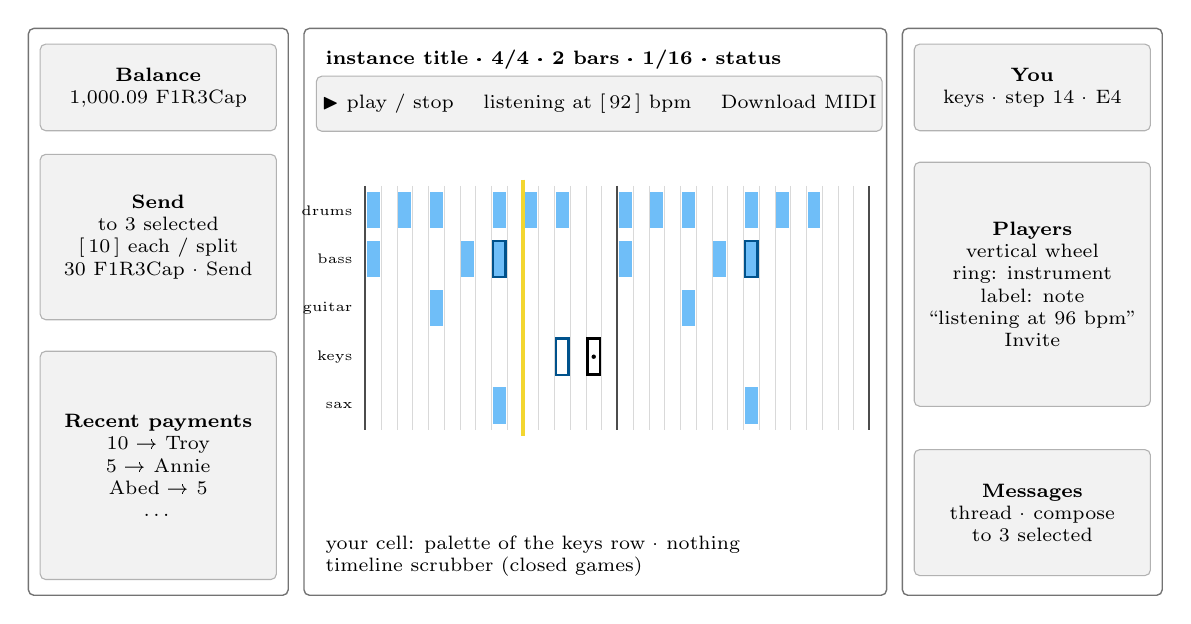
\begin{tikzpicture}[font=\scriptsize,
  col/.style={draw=black!55,line width=0.5pt,rounded corners=2pt},
  pane/.style={draw=black!30,rounded corners=2pt,fill=codebg,align=center,inner sep=2pt}]
  \draw[col] (0,0) rectangle (3.3,7.2);
  \draw[col] (3.5,0) rectangle (10.9,7.2);
  \draw[col] (11.1,0) rectangle (14.4,7.2);
  \node[pane,minimum width=30mm,minimum height=11mm] at (1.65,6.45) {\textbf{Balance}\\1,000.09 F1R3Cap};
  \node[pane,minimum width=30mm,minimum height=21mm] at (1.65,4.55) {\textbf{Send}\\to 3 selected\\{[}\,10\,{]} each / split\\30 F1R3Cap · Send};
  \node[pane,minimum width=30mm,minimum height=29mm] at (1.65,1.65) {\textbf{Recent payments}\\10 \textrightarrow{} Troy\\5 \textrightarrow{} Annie\\Abed \textrightarrow{} 5\\\ldots};
  \node[anchor=north west,font=\scriptsize\bfseries] at (3.65,7.05) {instance title · 4/4 · 2 bars · 1/16 · status};
  \node[pane,minimum width=70mm,minimum height=7mm,anchor=north west] at (3.65,6.6) {\(\blacktriangleright\) play / stop \quad listening at [\,92\,] bpm \quad Download MIDI};
  \begin{scope}[shift={(3.62,5.2)}]
    \foreach \r/\n in {0/drums,1/bass,2/guitar,3/keys,4/sax}{
      \node[anchor=east,font=\tiny] at (0.62,{-\r*0.62-0.31}) {\n};
    }
    \foreach \t in {0,...,32}{
      \pgfmathsetmacro{\x}{0.66+\t*0.2}
      \ifnum\t=16 \draw[black!70,line width=0.7pt] (\x,0) -- (\x,-3.1);
      \else\ifnum\t=0 \draw[black!70,line width=0.7pt] (\x,0) -- (\x,-3.1);
      \else\ifnum\t=32 \draw[black!70,line width=0.7pt] (\x,0) -- (\x,-3.1);
      \else \draw[black!15,line width=0.2pt] (\x,0) -- (\x,-3.1); \fi\fi\fi
    }
    \foreach \t/\r in {0/0,4/0,8/0,12/0,16/0,20/0,24/0,28/0,2/0,10/0,18/0,26/0,0/1,6/1,8/1,16/1,22/1,24/1,4/2,20/2,8/4,24/4}{
      \fill[brandsky!75] ({0.68+\t*0.2},{-\r*0.62-0.08}) rectangle ({0.84+\t*0.2},{-\r*0.62-0.54});
    }
    \draw[black,line width=1pt] ({0.68+14*0.2},{-3*0.62-0.08}) rectangle ({0.84+14*0.2},{-3*0.62-0.54});
    \fill[black] ({0.76+14*0.2},{-3*0.62-0.31}) circle (0.8pt);
    \foreach \t/\r in {8/1,24/1,12/3}{
      \draw[brandskydark,line width=0.9pt] ({0.68+\t*0.2},{-\r*0.62-0.08}) rectangle ({0.84+\t*0.2},{-\r*0.62-0.54});
    }
    \draw[brandyellow,line width=1.2pt] (2.66,0.08) -- (2.66,-3.18);
  \end{scope}
  \node[anchor=south west,font=\scriptsize,align=left] at (3.65,0.12) {your cell: palette of the keys row · nothing\\timeline scrubber (closed games)};
  \node[pane,minimum width=30mm,minimum height=11mm] at (12.75,6.45) {\textbf{You}\\keys · step 14 · E4};
  \node[pane,minimum width=30mm,minimum height=31mm] at (12.75,3.95) {\textbf{Players}\\vertical wheel\\ring: instrument\\label: note\\``listening at 96 bpm''\\Invite};
  \node[pane,minimum width=30mm,minimum height=16mm] at (12.75,1.05) {\textbf{Messages}\\thread · compose\\to 3 selected};
\end{tikzpicture}
\caption{The three columns. In the grid, the black-outlined cell with a dot is yours, dark sky
outlines mark the selected players' cells, and the yellow line is the playhead, which moves at
your own tempo.}
\label{fig:layout}
\end{figure}

\textbf{Left column: tokens.} As F1R3Pix: balance, the send control (\emph{each} or
\emph{split}, with the total), and the instance's recent payments.

\textbf{Centre column: the grid.} Above it, the transport: play and stop, the player's
listening tempo, and \emph{Download MIDI}. The grid shows rows labelled by instrument, bar lines
heavy, beat lines medium and columns light. Sounding cells carry their note's name. Void cells are hatched, seeded cells that no one has
taken have a dotted outline, and the cells of players who have left are dimmed. The player's
own cell is marked independently of colour, with a black outline and a dot. Clicking it opens
the note control. For the drum row, this is the twelve pieces as buttons. For a pitched row, it
is a keyboard strip spanning the row's range, with the scale's pitches enabled and the rest
disabled, plus \emph{nothing}. Hovering over a choice plays it
locally, which costs nothing and deploys nothing. Clicking another player's cell toggles their
selection, so the grid is also a selection surface.

\textbf{Right column: players.} As F1R3Pix. Each avatar's ring shows the player's instrument,
its label shows their current note, and its caption shows the tempo they are listening at (D7).
Selection drives board highlighting, message recipients and payment recipients together.

\begin{decision}{D10}{In what order does the wheel list players?}
\textbf{Agreed: by distance on the grid, with time wrapping, then by name or by recent
contact on request.} The distance between cells $(t,\rho)$ and $(t',\rho')$ is
$\min(|t-t'|,\,S-|t-t'|)+|\rho-\rho'|$, measured on the loop as a cylinder. The players
nearest a player sound at the same moment, which is where hits and chords are made, or just
before and after in the same row, which is where lines are made. Those are the players they
most need to talk to.
\end{decision}

\subsection{Sound}

\begin{itemize}[leftmargin=1.2em,itemsep=2pt]
\item \textbf{Rendering.} After each grid read, the core rebuilds the canonical score and its
  note list (timbre, pitch, onset, length, rests excluded), and the audio engine schedules the
  loop on the Web Audio clock at the listener's tempo. Tempo counts quarter notes, as F1R3Score's renderer
  does, so a column of $u$ whole notes lasts $240u/\mathit{bpm}$ seconds.
  Changes take effect at the next loop boundary, so the groove never stutters mid-bar.
\item \textbf{Timbres.} Everyone must hear the same instruments, so the client bundles one
  General MIDI sound set: the four programs and the kit, and nothing more. It \MUST{} be
  permissively licensed. FluidR3\_GM (MIT licence) is the candidate, cut to those samples.
  A device's own synthesizer is not used, because it would make the same pattern sound
  different to different players.
\item \textbf{Tempo.} The tempo control is local and immediate. It publishes through
  \code{listen} only after the control has rested (D7).
\item \textbf{MIDI.} \emph{Download MIDI} writes the loop as a Standard MIDI File at the
  listener's tempo, one track per timbre, matching what \code{f1r3score play --midi} writes for
  the same score.
\end{itemize}

\subsection{Behaviour}

\begin{itemize}[leftmargin=1.2em,itemsep=2pt]
\item \textbf{Freshness, pending sets and allowance.} As F1R3Pix, with \code{set} in place of
  \code{paint}. A note change sounds locally at once with a pending mark, and settles when a
  block includes it. While a set is in flight, further choices replace a single queued set.
  The allowance covers \code{seat}, \code{set}, \code{listen} and \code{say}.
\item \textbf{Accessibility.} No information is carried by colour alone: note names are
  printed in their cells, the player's own cell has an outline and a dot, and void, seeded
  and departed cells have hatching, dotting or dimming. Keyboard navigation follows cell
  indices, which is time order. The grid can be read aloud row by row, as note names and step
  numbers.
\item \textbf{Small screens.} Below 900 pixels, the columns become tabs, with the grid as the
  default tab. A grid wider than the screen scrolls horizontally, and the playhead keeps the
  current bar in view.
\end{itemize}

% ================================================================= 9
\section{Galleries}\label{sec:gallery}

\begin{decision}{D11}{What does a F1R3Beat play hold?}
\textbf{Options.} (a) Only patterns, as installed. (b) Only the history of a game. (c) Both,
as two gallery kinds, linked.

\textbf{Agreed: (c).} F1R3Skein distinguishes a \emph{performance} from the
\emph{tunes} a performer snips from it, and F1R3Beat has the same structure. A \code{session}
is the whole history of a game over a span of blocks, like a F1R3Pix play. A \code{pattern} is
the grid at one block, written as its canonical score. Patterns are what breed. Any participant
may cut a pattern from a session at any block, and the two are linked with \code{linkPlays}.
When the host closes an instance, the client offers to publish the session and its final
pattern together, with one prompt.
\end{decision}

\subsection{Patterns}

\begin{center}\small
\begin{tabularx}{\linewidth}{@{}l X@{}}
\toprule
part & content\\
\midrule
header & \code{title}; \code{digest} (R\ref{r:canon}); \code{meter}; \code{column}; \code{steps}; \code{tempo}, the publisher's listening tempo as a suggestion; \code{origin}, one of \code{game}, \code{bred} or \code{cross}; \code{parents}, the play ids of both parents for bred and crossed patterns, or of the seed for a seeded game; \code{operator} (\code{X} or \code{V}, \S\ref{sec:evolution}); \code{seed}, the block hash and epoch from which the generator was drawn; for a game pattern, \code{instance} and \code{blockHash}\\
body & CBOR \code{\{score: <canonical score text>, credits: [[cell, address], ...]\}}. Credits name the player seated at each sounding cell. Bred patterns have none, and their lineage credits their parents.\\
\bottomrule
\end{tabularx}
\end{center}

A pattern is verifiable. A game pattern's score can be rebuilt from \code{f1r3beat.grid} at
\code{blockHash}. A bred or crossed pattern can be rebuilt from its parents and its seed
(\S\ref{sec:verify}). In both cases its digest must match. Every published score plays in
\code{f1r3score} with no F1R3Beat code at all. The preview renderer draws the grid from the
score, and the full view plays it.

\subsection{Sessions}

A session's body is a byte array, the F1R3Pix encoding adapted to cells and notes:

\begin{lstlisting}
"F1BT"  u8 version = 1  u8 n  u8 d  u8 k  u8 bars  u32 from  u32 to   (column = 1/k)
u8 P  P × (u8 row, u8 code)        notes used in the span, in first-use order;
                                    code is the MIDI number
varint S  S × (varint Δh, u16 cell, u8 note)   sets in history order;
                                    note indexes the table, 255 = nothing
varint O  O × (u16 cell, 20 bytes address)      owners of the cells that appear
\end{lstlisting}

The full view plays a session as it was played: the loop runs, and the grid changes block by
block beneath the playhead.

\subsection{Engagement}

Views, plays and likes go through the Portal's \code{engage}. For sessions they rank the
gallery. For patterns they also set selection weights (D14).

% ================================================================= 10
\section{Evolution}\label{sec:evolution}

\subsection{The population}

The \emph{population} is a set of patterns kept in the environment under \code{("pop", p)}.
Membership is separate from publication: a pattern that leaves the population stays in the
gallery. Patterns join in three ways. A pattern published from a game joins at the next
epoch. A bred pattern joins when it is admitted. A crossed pattern joins once someone other
than the player who crossed it likes it (D15).

\subsection{Lines as streams}

Write a pattern of $S$ steps as its five lines $P=(P_\rho)_{\rho\in R}$, where
$R=(\mathit{drums},\mathit{bass},\mathit{guitar},\mathit{keys},\mathit{sax})$, and a line as
$L=[(p_1,d_1),\dots,(p_k,d_k)]$ with $\sum_j d_j=Su$. Following F1R3Skein, a line unzips into
two streams. In F1R3Beat the streams are cut differently, because the grid fixes time:

\begin{itemize}[leftmargin=1.2em,itemsep=2pt]
\item the \emph{rhythm} $\mathrm{rh}(L)=[(d_j,\,[p_j\ne\code{r}])]_j$, the durations together
  with which of them sound. It has $n(L)=\#\{j : p_j\ne\code{r}\}$ \emph{slots};
\item the \emph{melody} $\mathrm{mel}(L)$, the subsequence of the pitches $p_j\ne\code{r}$. For
  the drum row it is the sequence of kit pieces.
\end{itemize}

\textbf{Refilling.} Given a rhythm with $n$ slots, a melody of length $k$ and a generator $g$,
$\mathrm{refill}(\mathrm{rh},\sigma,g)$ is a line. If $k\ge n$, delete $k-n$ entries of
$\sigma$, chosen uniformly by $g$, keeping the order of the rest. If $k<n$, choose $n-k$ slots
uniformly by $g$ and make them rests. Then assign the melody to the remaining slots in order,
and normalise as in \S\ref{sec:canonical}, merging adjacent rests.

\subsection{The operators}

\begin{decision}{D12}{What are the children of two patterns?}
\textbf{Agreed: four children, two from each of two operators, as F1R3Skein has four.}
Agreed in review as workable for now.

\textbf{Rhythm and melody, row by row.} The cross of $A$ by $B$ keeps $A$'s rhythm and takes
$B$'s melody, independently in each row:
\[
  X(A,B)_\rho=\mathrm{refill}\bigl(\mathrm{rh}(A_\rho),\ \mathrm{mel}(B_\rho),\ g\bigr).
\]
This is F1R3Skein's first two children (Mother's pitches with Father's durations, and the
converse) applied to every line of the composition. A child has the length of its rhythm
parent. Every pitch stays in its row's range, because a melody never leaves its row.

\textbf{Voices exchanged at the composition.} For a vector $c\in\{0,1\}^5$ that is neither all
zeros nor all ones,
\[
  V(A,B;c)_\rho=\begin{cases}A_\rho & c_\rho=0\\ B_\rho & c_\rho=1\end{cases}
\]
takes whole lines from each parent. This operator cuts the score exactly where it composes,
at the parallel bars, where harmony comes from independence. It keeps each line intact, so a
bass figure and the kick it locks with can be inherited together if they come from the same
parent.

\textbf{The brood} of $A$ and $B$ is
$\{X(A,B),\ X(B,A),\ V(A,B;c),\ V(B,A;c)\}$, with one $c$ drawn for both voice children, so
the two are complements.

\textbf{Why not F1R3Skein's other two children.} F1R3Skein's third and fourth children rewrite
one parent's pitch stream as durations (in base 5) or its durations as pitches (in base 22).
On a grid, a duration must be a whole number of steps and a line's durations must fill the
pattern exactly, so rewritten digits would break the loop. The second axis of a beat is not a
change of alphabet but the composition of instruments, and $V$ recombines along it.
\end{decision}

\begin{figure}[h]
\centering
\begin{tikzpicture}
  \node[anchor=north west] at (0,0) {\begin{tikzpicture}\input{fig/mother-small.tex}\end{tikzpicture}};
  \node[anchor=north west,font=\scriptsize\bfseries] at (0.05,0.35) {$A$ (rhythm)};
  \node[anchor=north west] at (0,-3.2) {\begin{tikzpicture}\input{fig/father.tex}\end{tikzpicture}};
  \node[anchor=north west,font=\scriptsize\bfseries] at (0.05,-2.85) {$B$ (melody)};
  \node[anchor=north west] at (0,-6.4) {\begin{tikzpicture}\input{fig/child.tex}\end{tikzpicture}};
  \node[anchor=north west,font=\scriptsize\bfseries] at (0.05,-6.05) {$X(A,B)$};
\end{tikzpicture}
\caption{A cross. $A$ is the pattern of Figure~\ref{fig:mother}. The child keeps $A$'s rhythm in
every row and takes $B$'s melody: the drums keep $A$'s eight hits with $B$'s alternation of kick
and hat, The bass has five slots and $B$'s bass melody four pitches, so one slot, drawn by $g$, falls
silent, and so does one of the guitar's two slots. The saxophone
has two slots and $B$'s saxophone melody has three pitches, so one pitch, drawn by $g$, is
dropped. The keys have no slots, so $B$'s keys melody is lost.}
\label{fig:cross}
\end{figure}

The child of Figure~\ref{fig:cross}, in canonical form, is accepted by \code{f1r3score check}
(digest \code{fa30e9ae\ldots}):

\begin{lstlisting}[language=score,basicstyle=\ttfamily\scriptsize]
play line(base "drums", drums)       [ kick c1, r c1, chh c1, r c1, kick c1, r c1, chh c1, r c1,
                                     kick c1, r c1, chh c1, r c1, kick c1, r c1, chh c1, r c1 ]
   | line(base "bass", bass)         [ A2 c1, r c2, C3 c1, r c2, D3 c1, r c4, E3 c1, r c4 ]
   | line(base "guitar", guitar)     [ r c4, G3 c1, r c11 ]
   | line(base "keys", keys)         [ r c16 ]
   | line(base "sax", sax)           [ r c4, G4 c1, r c3, B4 c1, r c7 ]
\end{lstlisting}

\subsection{Shapes and mutation}

\begin{decision}{D13}{Which patterns can breed, and where does variation come from?}
\textbf{Agreed.}

\textbf{Shapes are species.} Two patterns breed only if they have the same time signature and
the same column (D5). Lines in different meters or subdivisions do not share a grid, and splicing them would yield polymeter. That
is interesting, but it is a different game (\S\ref{sec:future}).

\textbf{Lengths are equalised by silent bars.} $X$ needs no equalising, because the child takes
its rhythm parent's length. $V$ needs both parents to be the same length. The shorter is padded
with silent bars, inserted at bar boundaries chosen uniformly by $g$, until the lengths match.
This is F1R3Skein's padding of the shorter snippet with rests at random places, moved to the
bar, which is the unit at which a beat can grow without breaking its pulse.

\textbf{Mutation.} Variation comes from refilling (slots silenced, pitches dropped) and from
padding, as it does in F1R3Skein, and from nothing else by default. A point mutation, which
replaces a sounding pitch with one drawn uniformly from its row's palette at rate $\mu$ per
note, is specified with $\mu=0$. It can be turned on once Phase~6 shows whether the population
loses diversity without it.
\end{decision}

\subsection{Selection and culling}

\begin{decision}{D14}{Which patterns breed, and which leave?}
\textbf{Agreed.} The weight of a pattern is
$w=1+\mathit{plays}+3\cdot\mathit{likes}$, counted from the Portal's engagement by distinct
addresses, as the F1R3Skein prototype counted it. At each epoch:
\begin{enumerate}[leftmargin=1.4em,itemsep=1pt]
\item Draw $A$ from the population with probability proportional to $w$.
\item Draw $B$, proportionally to $w$, from the members of $A$'s species other than $A$. If
  there are none, draw $A$ again from the species with at least two members, and if there are none,
  the epoch breeds nothing.
\item Compute the brood. Drop any child whose digest is already in the population, or equals
  another child's.
\item Admit the brood. Then draw $k$ uniformly from $\{1,2,3\}$, and remove the $k$ members
  with the least weight among those at least three epochs old. Ties go to the older member,
  then to the smaller digest. The population is never culled below 16 members.
\end{enumerate}
The grace period is new. Without it, a child, whose engagement starts at nothing, is the
likeliest member to be culled at the very epoch that admits it, so selection could never see
it.
\end{decision}

\subsection{Who breeds}

\begin{decision}{D15}{Who runs reproduction?}
\textbf{Options.} (a) A breeder service runs epochs. (b) Players cross patterns they choose.
(c) Both.

\textbf{Agreed: (c).} \textbf{Epochs} run every $E$ blocks, with $E$ set in Phase~4 so
that an epoch is about a day. The breeder computes the epoch from public data and signs two
moves with the breeder key: \code{admit(epoch, children)} and \code{cull(epoch, members)}. The
environment checks only the key and that epochs increase. Correctness is checked by anyone who
recomputes (\S\ref{sec:verify}). The breeder key is registered by the F1R3FLY.io Cooperative,
which governs the registry.

\textbf{Crosses} let a player choose two patterns of the same species in the gallery and breed
them. The client computes the brood and publishes the four children, with origin \code{cross},
in one prompt. A crossed child enters the population only after someone other than the crosser
likes it. That keeps the population from filling with one player's crosses, and it means a
human other than the crosser has heard the child before it can breed.
\end{decision}

\subsection{Randomness and verification}\label{sec:verify}

\req{r:seed}~The generator $g$ for an epoch \MUST{} be xoshiro256** seeded through SplitMix64,
as F1R3Score's \code{score-chance} crate implements it. The seed \MUST{} be the first eight bytes,
read little-endian, of
\[
  \mathrm{blake2b256}\bigl(\text{\code{"f1r3beat/breed/v1"}}\ \|\ H\ \|\ \mathit{epoch}\bigr),
\]
where $H$ is the hash of the epoch's block, and engagement \MUST{} be read as of that block.
For a brood, the seed is extended with the two parents' digests. For a cross, $H$ is a block
named in the children's headers, which \MUST{} be at most 50 blocks older than the block that
includes the publication.

\req{r:draws}~Draws \MUST{} be taken in this order: selection; padding positions, in
increasing bar order; $c$, as a uniform integer in $[1,30]$ read in binary with the drum row as
the most significant bit; then the refills of $X(A,B)$ in row order, then those of $X(B,A)$. A
uniform integer below $m$ is drawn by rejection: take a 64-bit output $x$, retry while
$x\ge m\lfloor 2^{64}/m\rfloor$, and answer $x\bmod m$. A uniform choice of $j$ positions out of
$m$ is the first $j$ entries of a Fisher--Yates shuffle of $0,\dots,m-1$, sorted.

Given those rules, an epoch is a pure function of the chain. \code{f1r3beat-breed verify
--epoch e} recomputes it from the population, the engagement and the block hash, and compares
the digests admitted and culled with those the breeder key wrote. A breeder that cheats is
caught by anyone who runs it.

\subsection{Patterns back into play}

\begin{decision}{D16}{Can a game start from a pattern?}
\textbf{Agreed: yes.} A host may seed a new instance from any pattern of the same shape:
meter, column and length. The client converts the score into cell notes, which is exact
because every note is one column long. The configuration's \code{seed} carries the play id, the digest and the cell
notes. The environment writes them as cells with no owner. A player seated on a seeded cell
inherits its note and can change it. Patterns published from the game list the seed as their
parent.

This closes the loop. Players make patterns, the gallery's engagement selects among them,
reproduction recombines them, and a recombined pattern can become the starting point for
people to play again. The evolution never runs without humans in it.
\end{decision}
% ================================================================= 11
\section{Security and abuse}\label{sec:security}

Everything in F1R3Pix's table applies, with \code{set} for \code{paint}. The rows below are
the threats F1R3Beat adds.

\begin{center}\small
\begin{tabularx}{\linewidth}{@{}>{\raggedright\arraybackslash}p{40mm} X@{}}
\toprule
threat & answer\\
\midrule
Setting another player's cell & Impossible: \code{set} names no cell and writes only the caller's seat.\\
Injection through notes & The environment accepts only palette members or \code{Nil}. The score bridge writes score text only from fixed tables of row, pitch, kit and duration names, never from strings it was given.\\
A dishonest breeder & The breeder key can only admit and cull. Every epoch is recomputable (R\ref{r:seed}, R\ref{r:draws}), and \code{verify} exposes a forgery. The Cooperative can rotate the key.\\
Engagement farming & Weights count distinct addresses, and each address engages once per kind. Sybil addresses still cost phlo and a profile. Tournaments and stake-weighted engagement are the stronger answers, and are later work.\\
Grinding a cross's seed & The block named for a cross must be at most 50 blocks old, so a crosser chooses among at most 50 broods. A crossed child cannot breed until someone else likes it.\\
Flooding the population & Game patterns join once per publication. Crosses need another player's like. Culling keeps the size bounded.\\
Metadata & Listening tempo is public by design (D7). Message metadata is public as in F1R3Pix.\\
\bottomrule
\end{tabularx}
\end{center}

% ================================================================= 12
\section{Manifest and conformance}\label{sec:manifest}

\begin{lstlisting}
{ "id": "f1r3beat", "name": "F1R3Beat",
  "tagline": "One step each. Make a groove together.",
  "entry": "<entry-base>/f1r3beat/", "platforms": ["web"],
  "env": "rho:id:...",                     // unchanged URI; environment version raised
  "templates": [ "f1r3beat.seat", "f1r3beat.set", "f1r3beat.listen", "f1r3beat.say",   // play
                 "f1r3beat.grid", "f1r3beat.seats", "f1r3beat.log", "f1r3beat.mail",
                 "f1r3beat.outbox", "f1r3beat.population" ],                         // explore
  "capabilities": ["pay", "open"],
  "galleries": [ { "kind": "pattern", "renderer": "<entry-base>/f1r3beat/preview/pattern.html" },
                 { "kind": "session", "renderer": "<entry-base>/f1r3beat/preview/session.html" } ],
  "contactsDialogue": true, "readerTier": false, "minProtocol": 2 }
\end{lstlisting}

The templates \code{f1r3beat.toggle}, \code{f1r3beat.tempo} and \code{f1r3beat.state} are
retired. \code{admit} and \code{cull} are not game templates. They are signed only by the
breeder key, from the breeder, and are absent from the manifest.

\textbf{Conformance tests} extend the Portal's and F1R3Pix's:

\begin{itemize}[leftmargin=1.2em,itemsep=1pt]
\item the environment and every template parse with the node's own parser (\code{rholint}), and
  every play template binds no deployer authority;
\item cell indices, seating (random, claim and row), palettes and session encodings
  round-trip against shared vectors in Rust and TypeScript;
\item for every grid vector, the Rust and TypeScript bridges produce the same canonical text.
  \code{f1r3score check} accepts it with the recorded digest, and the notes of \code{f1r3score
  play --format json}, rests excluded, are exactly the onsets the grid denotes. This runs in CI
  against F1R3Score pinned at a stated revision;
\item breeding vectors: for given parents, block hash and epoch, the brood's digests, in Rust
  and TypeScript. \code{verify} accepts a correct epoch and rejects one with a single child
  altered;
\item end to end against the mock node: seat, set, listen, say, open, pay, publish a pattern and
  a session, rebuild both from the chain, run an epoch, and verify it.
\end{itemize}

% ================================================================= 13
\section{F1R3Gaze}\label{sec:gaze}

F1R3Beat needs the two capabilities F1R3Pix adds to the Portal's \code{GAZE-MAPPING.md}:
\code{pay}, attenuated to the instance's participants, and \code{open}, bound to the game and
instance. It needs one more, which no game has needed so far: \emph{sound}. A f1r3lang page in
F1R3Gaze has no audio output. The natural capability takes note records (timbre, pitch, onset,
length) and plays them against the browser's clock at a given tempo. Those are the records
F1R3Score's renderer already produces, and its live-MIDI path already schedules them in wall
time. A sound capability shaped that way would let a f1r3lang page play any F1R3Score
performance, not only F1R3Beat's. \code{GAZE-MAPPING.md} should gain the row when Phase~3 lands.

% ================================================================= 14
\section{Development plan}\label{sec:plan}

\begin{center}\small
\begin{tabularx}{\linewidth}{@{}>{\raggedright\arraybackslash}p{28mm} X >{\raggedright\arraybackslash}p{44mm}@{}}
\toprule
phase & work & done when\\
\midrule
1 · Environment & New \code{f1r3beat.rho} body; \code{seat}, \code{set}, \code{listen}, \code{say}; reads; palettes; manifest; seating and palette vectors. & Parses; template rules pass; mock-node tests of every move and read.\\
2 · Score bridge & Rust crate (grid to canonical score, score to notes, MIDI) and its TypeScript twin; grid vectors; the CI job against \code{f1r3score}. & Both bridges agree on every vector, and \code{f1r3score} agrees with both.\\
3 · Client & Core and views; grid, note control, transport; audio engine and the cut-down sound set; pending sets; accessibility; tabs. & Plays a full game against the mock node with five simulated players, audibly.\\
4 · Live shard & Install; measure phlo for each move and read; set the allowance, the 64-step bound and the epoch length $E$. & One live game of at least eight players, start to close.\\
5 · Galleries & Pattern and session encodings; publishing at close; cutting patterns from sessions; renderers; engagement. & A closed game publishes both kinds, and both rebuild from the chain.\\
6 · Evolution & Breeder crate on the score bridge and F1R3Score's \code{score-chance}; population moves; crosses in the client; \code{verify}; seeding instances from patterns. & Ten epochs on a test shard, each verified independently; a seeded game played from a bred pattern.\\
Later & Uploaded samples and timbres; polymeter; a timed-touch keyboard form; tournaments; the F1R3Gaze version. & \\
\bottomrule
\end{tabularx}
\end{center}

Phases 1 and 2 can proceed together, and Phase 3 can begin against stubs. One dependency
outside this repository constrains the plan. F1R3Score's \code{DESIGN.md} records that its
\code{wasm32} build has not been verified. Until it is, the client runs the TypeScript bridge,
Rust runs only in the breeder and in \code{verify}, and the CI job of Phase~2 keeps the two
honest against \code{f1r3score} itself.

% ================================================================= 15
\section{Decisions}\label{sec:decisions}

\begin{center}\small
\begin{tabularx}{\linewidth}{@{}l>{\raggedright\arraybackslash}p{38mm}X@{}}
\toprule
 & question & decision (all agreed in review, 6 October 2026)\\
\midrule
D1 & Grid size, empty cells & Shape and capacity fixed at creation (default 4/4 in sixteenths, 2 bars, 32 seats; at most 64 steps); unseated cells are void and silent.\\
D2 & Seating & Random and verifiable by default; claim and row seating as host options.\\
D3 & A player who leaves & Keeps the cell, still sounding, dimmed.\\
D4 & \textbf{Settled.} Pitch & One pitch per cell from the row's palette; the drum set is one row whose palette is the kit; optional host scale.\\
D5 & \textbf{Settled.} Note length & Every note lasts one column; the column, the subdivision of the beat, is chosen at setup.\\
D6 & Phases & Lobby: seat, listen, talk, pay. Active: also set. Closed: read only.\\
D7 & \textbf{Settled.} Tempo & A default per instance; each player listens at their own tempo, shown as part of their description; tempo is not part of the pattern.\\
D8 & Messages and payments & As F1R3Pix, with F1R3Beat's domain strings.\\
D9 & \textbf{Settled.} Notation & Patterns are F1R3Score scores, a parallel composition of five lines, in a canonical form whose digest is the pattern's identity.\\
D10 & Wheel order & Nearest on the looped grid first.\\
D11 & Galleries & \code{session} (history) and \code{pattern} (a moment as a score), linked.\\
D12 & Children & Four: rhythm-by-melody crosses both ways, and two complementary voice exchanges; workable for now.\\
D13 & Shapes and mutation & Same meter and column only; silent bars pad length; variation from refilling and padding; point mutation off.\\
D14 & Selection and culling & Weight $1+\mathit{plays}+3\cdot\mathit{likes}$; cull 1--3 of the least weighted after a three-epoch grace; floor of 16.\\
D15 & Who breeds & Epochs by a recomputable breeder, and player crosses that enter on another player's like.\\
D16 & Seeding & A game may start from a pattern; seeded cells are inherited by whoever sits there.\\
\bottomrule
\end{tabularx}
\end{center}

\subsection{Out of scope for version 1}\label{sec:future}

Uploaded samples and timbres, which the March design anticipates, together with instances that
choose their rows from timbres stored on the shard. Also out of scope: notes longer than one column (ties across cells); a second pass on the
reproduction operators (D12); chords and velocity within a cell; swing; polymeter and breeding across meters; tempo as a graded dimension of the
score; a keyboard form of the score, once F1R3Score has a touch that waits for its stamp;
tournaments; hidden recipient lists and reports, as in F1R3Pix; and the F1R3Gaze version.

\end{document}
